\documentclass{article}
\usepackage[utf8]{inputenc}
\usepackage{polyglossia}
\usepackage[table]{xcolor}
\usepackage{graphicx}
\usepackage{multirow}
\usepackage[figurename=Attēls]{caption}
\usepackage{caption}
\usepackage{enumitem}
\usepackage{tikz}
\usetikzlibrary{shapes,arrows,shadows}
\usepackage{amsmath,bm,times}
\usepackage{systeme}
\usepackage{pdflscape}
\usepackage[american,siunitx]{circuitikz}
\usetikzlibrary{calc,positioning}
\usetikzlibrary{shapes.geometric}
\usepackage{diagbox}
\usepackage{float}
\usepackage{fontspec}
\usepackage{hyperref}
\usepackage{enumitem}
\usepackage{listings}
\usepackage{xcolor}

\definecolor{codegreen}{rgb}{0,0.6,0}
\definecolor{codegray}{rgb}{0.5,0.5,0.5}
\definecolor{codepurple}{rgb}{0.58,0,0.82}
\definecolor{backcolour}{rgb}{0.95,0.95,0.92}

\lstdefinestyle{mystyle}{
    backgroundcolor=\color{backcolour},
    commentstyle=\color{codegreen},
    keywordstyle=\color{magenta},
    numberstyle=\tiny\color{codegray},
    stringstyle=\color{codepurple},
    basicstyle=\ttfamily\footnotesize,
    breakatwhitespace=false,
    breaklines=true,
    captionpos=b,
    keepspaces=true,
    numbers=left,
    numbersep=5pt,
    showspaces=false,
    showstringspaces=false,
    showtabs=false,
    tabsize=2
}

\lstset{style=mystyle}

\usepackage{geometry}
\geometry{a4paper,total={170mm,257mm},left=20mm,top=20mm,}

\setsansfont{Arial}

\DeclareCaptionLabelFormat{nospace}{#2#1}
\captionsetup[figure]{labelfont={bf},name={. attēls},labelformat=nospace,labelsep=period}

\renewcommand{\labelenumii}{\theenumii}
\renewcommand{\theenumii}{\theenumi.\arabic{enumii}.}
\renewcommand{\labelenumiii}{\theenumiii}
\renewcommand{\theenumiii}{\theenumii\arabic{enumiii}.}



\newcommand{\mymeter}[2] 
{  % #1 = name , #2 = rotation angle
%\begin{scope}[transform shape,rotate=#2]
\begin{scope}[transform shape]
%\draw[thick] (#1)node(){$\mathbf V$} circle (11pt);
\draw[thick] (#1)node(){$\mathbf #2$} circle (11pt);
%\draw[rotate=45,-latex] (#1)  +(-17pt,0) --+(17pt,0);
\end{scope}
}

\begin{document}

\begin{titlepage}
\begin{center}
\large{Rīgas Tehniskā universitāte \\\vspace{3mm} Elektronikas un telekomunikāciju fakultāte \\\vspace{3mm} Elektronikas pamatu katedra}
\end{center}

\vspace{3cm}

\begin{center}
Datormācība (speckurss)\\10. - 11. nodarbība
\end{center}

\begin{center}
\textbf{Vienkāršu elektrisku shēmu modelēšana}
\end{center}

\vspace{5cm}

\begin{flushright}
Grupas Nr. REBM01
 \end{flushright}

 \begin{flushright}
Emīls Vizulis
 \end{flushright}
 
 \begin{flushright}
Studenta apliecības Nr. 191REB136
 \end{flushright}

\vfill
\begin{center}
\scshape{Rīga,2020}
\end{center}
\end{titlepage}
\renewcommand*\contentsname{Saturs}
\tableofcontents
\newpage

\vspace{0.25cm}
    
\textbf{Darba mērķi}
\begin{itemize}
    \item Iemācīties veidot dokumentus, kas labi izskatās
    \item Iemācīties kompilēt LaTeX dokumentus lokāli
    \item Nostiprināt zināšanas par Git.
\end{itemize}

\section{Ievads}


Šajā nodarbībā tiks veidots LaTeX fails, kurā tiks aprakstītas un ar bildēm papildinātas 9. nodarbībā veiktās darbības.

9. Nodarbībā mēs iemācījāmies ar gEDA programmām veikt vienkāršu shēmu simulāciju.

Šīs 9. nodarbībā iegūtās zināšanas mēs izmantosim, lai uzrakstītu aprakstu kā veikt simulāciju, kādas darbības jāveic, lai to izdarītu veiksmīgi.

Shēmas simulācijai veicamās darbības
Lai veiktu shēmas simulāciju, tā vispirms ir jauzīmē un jāapstrādā, lai programmās varētu apstrādāt tām piešķirto informāciju. Veicot datu sagatavošanu apstrādei ir jāzin noteiktas lietas, lai darbs notiktu veiksmīgi un nebūtu jāsaskaras ar liekām problēmām.

\section{Shēmas zīmēšana, jeb GSchem daļa}

Sāksm ar shēmas zīmēšanu, šim darbam mēs izmantosim 'gschem' programmu, to var palaist ierakstot konsolē {\large \textsf{'gschem'}}.

\vspace{3mm}
\begin{center}
    Atvērsies šāds logs:
\end{center}

\begin{figure}[H]\centering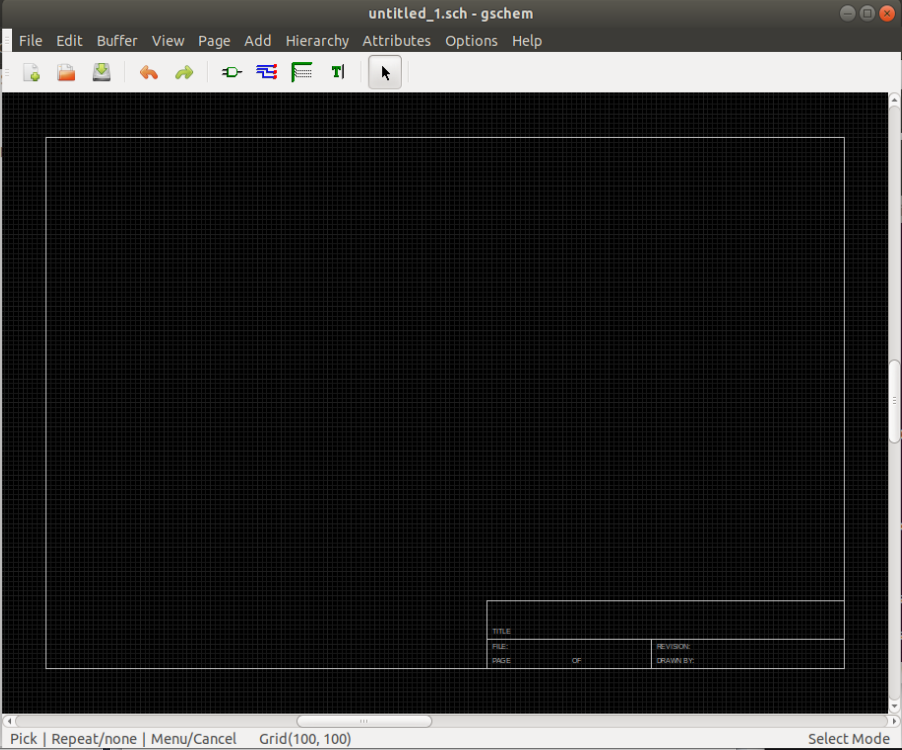
\includegraphics[width=0.80\textwidth]{pictures/spice/Logs.PNG}\caption{Shēmas zīmēšanas vides logs}\label{picture:10lw1p}\end{figure}

\subsection{Komponenšu izvietošana}

Vispirms veiksim shēmas zīmēšanu un tikai pēctam veiksim vērtību ievadīšanu. Lai sāktu zīmēt shēmu, mums tajā ir jāievieto komponentes, tās ver atrast zem pogas {\large \textsf{'Add component'}}, kas atvērs sarakstu ar daudzām komponentēm. Lai vieglāk būtu atrast komponenti kura mums ir nepieciešama, var izmantot meklētāju jeb filtru {\large \textsf{'Filter:'}} tajā ierakstot komponentes nosaukumu angļu valodā.

\begin{figure}[H]\centering
\includegraphics[width=0.50\textwidth]{pictures/spice/Components.PNG}\caption{Ikona, lai sāktu izvietot komponents}\label{picture:10lw2p}\end{figure}
\begin{figure}[H]\centering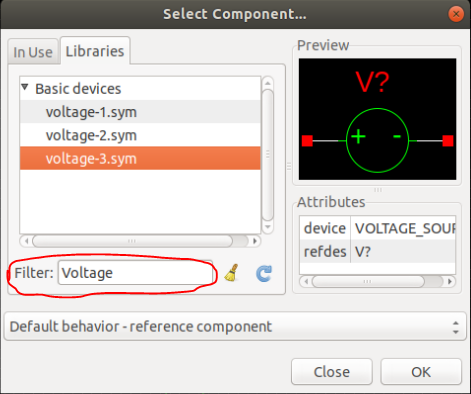
\includegraphics[width=0.50\textwidth]{pictures/spice/ComponentFilter.PNG}\caption{Komponenšu izvēles logs ar meklētāju}\label{picture:10lw3p}\end{figure}

\subsection{Komponenšu savienošana}

Kad komponentes ir izvietotas vēlamajās vietās, tās jāsavieno ar vadiem, jeb šajā gadījumā tie ir iedomāti savienojumi, kuriem nav pretestības. Vadus sāk zīmēt nospiežot uz pogas {\large \textsf{'Add netsmode'}}, kas pārslēgs rezīmu lai sāktu zīmēt vadus. Tagad nospiežot jebkurā vietā uz shēmas (sākumpunktā) un pēctam citā (beigu punktā) tiks uzzīmēts vads starp šiem diviem punktiem. Tāpēc, lai savienotu komponentes, kā sākumpunktu izmantosim vienas komponentes kādu no izvadiem un kā beigu punktu kādas citas komponentes kādu no izvadiem.

\begin{figure}[H]\centering
\includegraphics[width=0.50\textwidth]{pictures/spice/Netnodes.PNG}\caption{Ikona, lai sāktu zīmēt vadus}\label{picture:10lw4p}\end{figure}

\begin{center}
\begin{tabular}{cc}
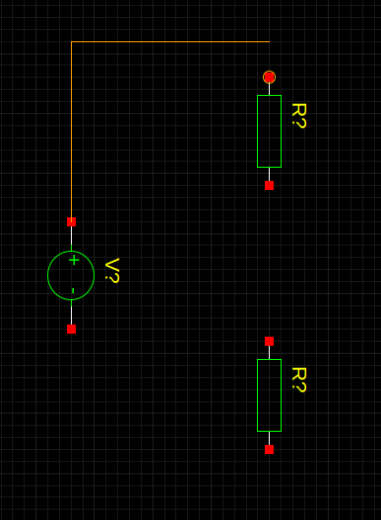
\includegraphics[width=0.326\textwidth]{pictures/spice/Zimesana.PNG}\caption{Zīmēšanas sākums}\label{picture:10lw5p}     &  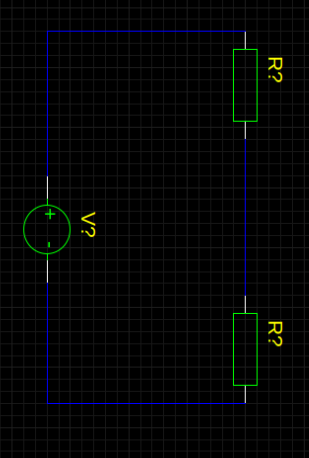
\includegraphics[width=0.30\textwidth]{pictures/spice/ZimesanaPabeigta.PNG}\caption{Pabeigta komponenšu savienošana}\label{picture:10lw6p}\\
5. attēls. Zīmēšanas sākums & 6. attēls. Pabeigta komponenšu savienošana
\end{tabular}    
\end{center}

\setcounter{figure}{6}

\subsection{Paramatru vērtību piešķiršana}

Kad shēma ir uzzīmēta, ir nepieciešams norādīt elementu vērtības. Lai to varētu sākt darīt vispirms jāizslēdz vadu zīmēšanas režīms, ja to neizdarīsim, mēģinot atlasīt elementu kuram piešķirsim vērtības, mēs turpinātu zīmēt vadus, ko šobrīd mums īsti vairs nevajag. To var izdarīt ar pogu kuras ikona ir tāda pati, vai līdzīga peles kursoram (uzbraucot uz šīs pogas parādīsies {\large \textsf{'Select mode'}}). Tagad kad esam izslēguši vadu zīmēšanas režīmu, varam sākt vērtību piešķiršanu elementiem.

\begin{figure}[H]\centering
\includegraphics[width=0.50\textwidth]{pictures/spice/Kursors.PNG}\caption{Ikona, lai sāktu izvietot komponents}\label{picture:10lw7p}\end{figure}

Divreiz noklikšķinot uz elementa atvērsies logs kurā būs redzam dažādi tā raksturojošie parametri. Atribūts {\large \textsf{'refdes'}} norāda šī elementa norādīto nosaukumu, nomainot šī atribūta vērtību mēs elementam piešķirsim nausaukumu, kuru mēs pēctam spēsim atpazīt (Piemēram 'V1' - avotam, 'R3' - pretestībai utt.). Diemžēl, mums nav vēl atribūta kurš norāda uz elementa nomināla vērtību, tādēļ to pievienosim. Lai pievienotu nomināla vērtību, atribūtu sarakstā atradīsim atribūtu kurš norāda elementa vērtību {\large \textsf{'Value'}} un kad esam atlasījuši šo atribūtu iedosim viņam skaitlisko vērtību, kad tas ir izdarīts nospidīsim {\large \textsf{'Add'}} un būsim elementam piešķīruši nepieciešamās vērtības (Sarežģītākiem elementiem varētu būt arī nepieciešams piešķirt vairāk vērtību). To pašu atkārtosim arī citiem elementiem.

\begin{center}
\begin{tabular}{cc}
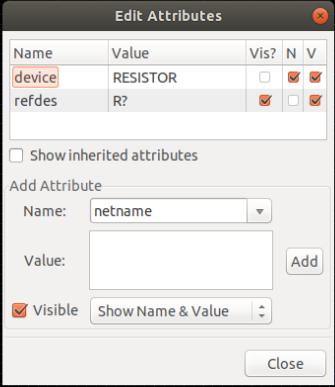
\includegraphics[width=0.326\textwidth]{pictures/spice/Parametri.PNG}\caption{Komponentes atribūti}\label{picture:10lw8p}     &  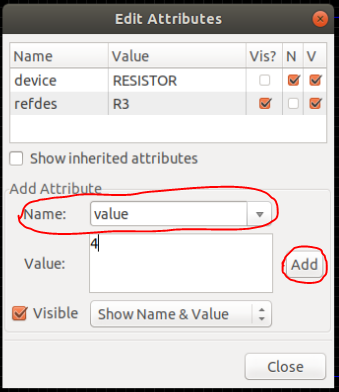
\includegraphics[width=0.326\textwidth]{pictures/spice/ParametrVertiba.PNG}\caption{Atribūtu pievienošana}\label{picture:10lw9p}\\
8. attēls. Komponentes atribūti & 9. attēls. Atribūtu pievienošana
\end{tabular}    
\end{center}

\setcounter{figure}{9}

\subsection{Shēmas attēla izvadīšana}

GSchem piedāvā arī izvadīt shēmas attēlu, kuru varēs apskatīties bez paša GSchem klātbūtnes. Lai to izdarītu programmas loga augšpusē uzpiedīsim uz file, kas atvērs izvelni. Šajā izvēlnē nospiedīsim {\large \textsf{'print...'}}. Tik atvērts lodziņš kurā tik piedāvādas dažādas attēla izvadīšanas opcijas. Mums tikai būs nepieciešams atlasīt, lai tiek izvadīts uz failu {\large \textsf{'File:'}} un nospiežot print, tiks izveidots fails ar shēmas attēlu.

\begin{center}
\begin{tabular}{cc}
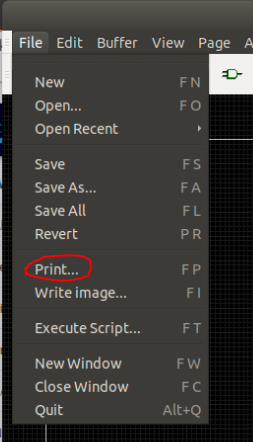
\includegraphics[width=0.2451\textwidth]{pictures/spice/Print.PNG}\caption{Attēla izvadīšana (Print)}\label{picture:10lw10p}     &  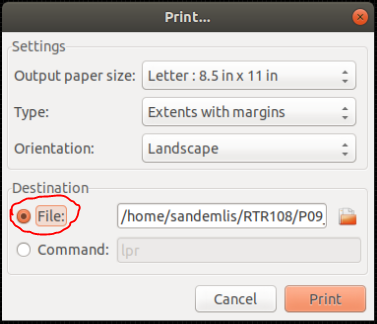
\includegraphics[width=0.5\textwidth]{pictures/spice/PrintFile.PNG}\caption{Opcija, lai izvadītu uz failu}\label{picture:10lw11p}\\
10. attēls. Attēla izvadīšana (Print) & 11. attēls. Opcija, lai izvadītu uz failu
\end{tabular}    
\end{center}

\setcounter{figure}{11}

\section{Elementu-mezglu faila izveidošana (*.net)}

Šis fails (saraksts) ir nepieciešams, lai mēs no izveidotās shēmas varētu veikt simulācijas, tas saturēs elementu vērtības un meglus pie kuriem šie elementi ir savienoti. Šīs darbības veikšanai izmantosim komandu {\large \textsf{'gnetlist'}} Tālāk tiks norādīts komandas pielietošanas piemērs, lai šo darbību varētu veikt:

\begin{lstlisting}
gnetlist -g spice -o [fails kur] [fails no kura] 
\end{lstlisting}

{\large \textsf{"[fails kur]"}} norāda komandai failu, kurā tiks veikts elementu-mezglu saraksts \newline
{\large \textsf{"[fails no kura]"}} norāda shēmas failu, no kura tiks veidots elementu-mezglu saraksts (parasti beidzas ar .net)

\vspace{5mm}
Ja shēmā viss tika izdarīts pareizi, tad jauniegūtajā faila saturam jaizskatās līdzīgi šim.
\vspace{2mm}
\begin{figure}[H]\centering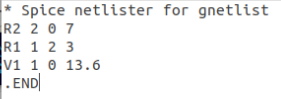
\includegraphics[width=0.5\textwidth]{pictures/spice/ElementuMezgluSaraksts.PNG}\caption{Elementu-Mezglu saraksts}\label{picture:10lw12p}\end{figure}

\section{Shēmas simulācijas veikšana}

Lai veiktu shēmas simulāciju ir jāpalaiž NGSpice ierakstot {\large \textsf{'ngspice'}} konsolē Kad NGSpice ir palaists būs jāieraksta dažas komandas kuras tiks izmantotas, lai iegūtu simulācijas recultātus.

Šīs komandas jāraksta ir šādā secībā, lai veiktu simulāciju

\begin{lstlisting}
source [fails] 
tran [solis] [beigas] [saakums]
\end{lstlisting}

Komanda {\Large \textsf{'source'}} norāda failu, kuram tiks veikta simulācija, šis fails jānorāda {\large \textsf{"[fails]}} vietā. Šājā failā, kuru izmantos, lai veiktu simulāciju, ir jābūt mezlu-elementu sarakstam.\newline
Komanda 'tran' veiks simulāciju laika posmā, \newline{\large \textsf{"[solis]"}} norāda ik pēc cik ilga laika tiks veikta mērījumu fiksēšana, \newline{\large \textsf{["beigas"]}} norāda beigu laiku, kad beigs veikt mērījumu piefiksēšanu, \newline un {\large \textsf{["sākums"]}} norāda laiku, kurā sākt veikt mērījumu piefiksēšanu 

Norādot laiku, ja netiek norādītas mērvienības, ievadītie cipari tiek uzskatīti kā sekundes, bet ja vēlas norādīt mērīšanas intervālu mazākā diapazonā, piemēram ja ir straujas izmaiņas, būs laiks jānorāda ar mērvienību, piemēram ms, us, utt.

\begin{figure}[H]\centering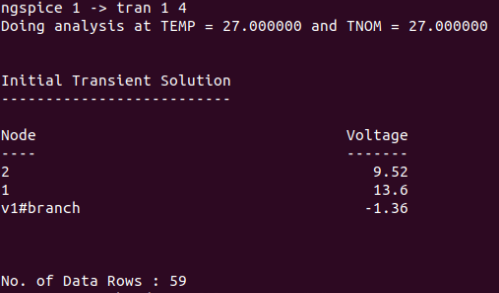
\includegraphics[width=0.5\textwidth]{pictures/spice/Simulacija.PNG}\caption{Simulācija}\label{picture:10lw13p}\end{figure}


Tālāk norādītās komandas tiek izmantotas, lai izvadītu veikto simulāciju grafikus.

\begin{lstlisting}
plot "[mezgls]"                     vai arii     plot "[mezgls1]" "[mezgls2]" 
hardcopy [fails kur] "[mezgls]"     vai arii     hardcopy [fails kur] "[mezgls1]" "[mezgls2]"
\end{lstlisting}

Komanda plot parādīs uz ekrāna grafiku, bet komanda hardcopy grafiku izvadīs failā.

\begin{center}
\begin{tabular}{cc}
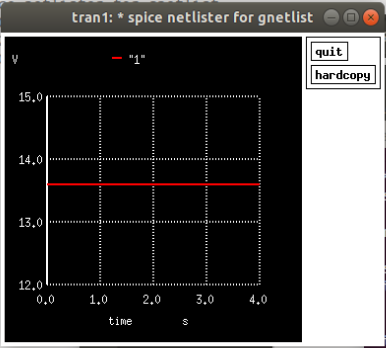
\includegraphics[width=0.4\textwidth]{pictures/spice/PlotGrafiks.PNG}\caption{Plot izvadītais grafiks}\label{picture:10lw14p}     &  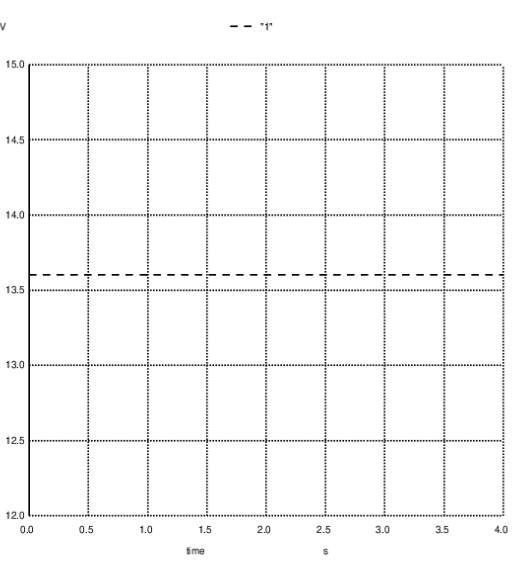
\includegraphics[width=0.35\textwidth]{pictures/spice/HardcopyGrafiks.PNG}\caption{Hardcopy izvadītais grafiks}\label{picture:10lw15p}\\
14. attēls. Plot izvadītais grafiks & 15. attēls. Hardcopy izvadītais grafiks
\end{tabular}    
\end{center}

\setcounter{figure}{15}

\end{document}